\section{关于同源/跨源OPD实验的更多讨论}

\begin{figure*}[t]
    \centering
    \begin{subfigure}[b]{0.48\linewidth}
        \centering
        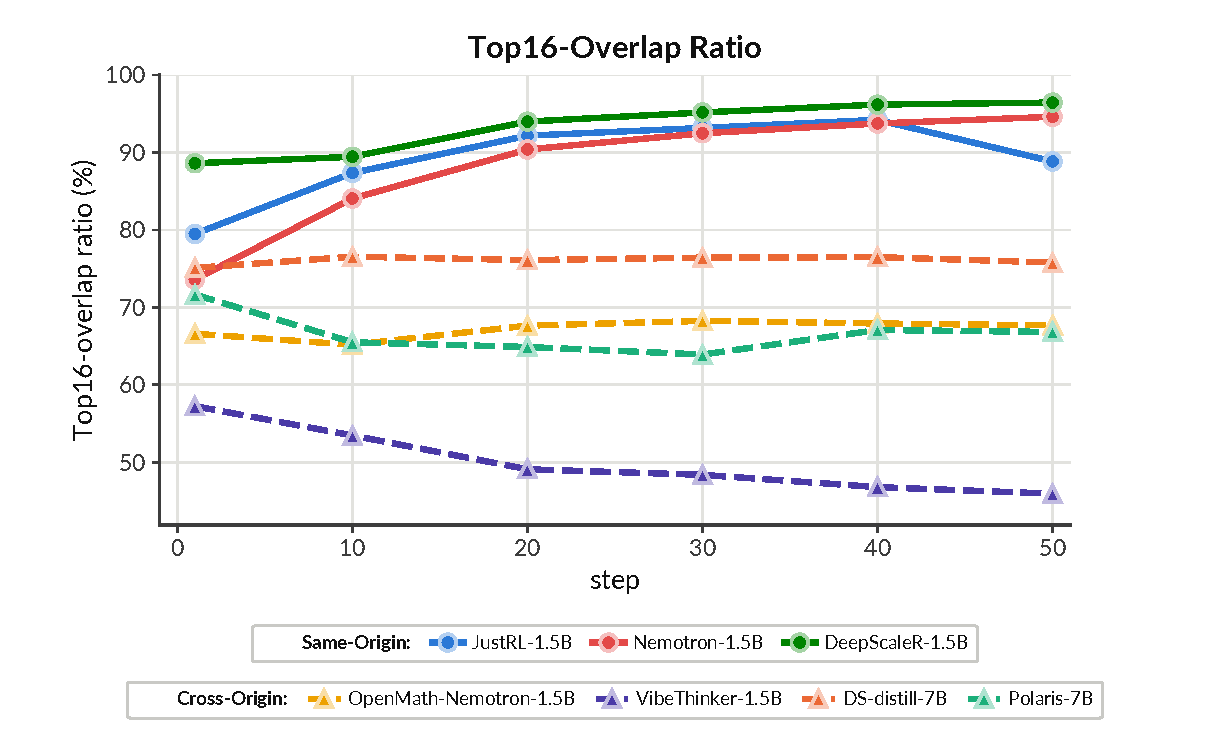
\includegraphics[width=\linewidth]{latex/figures/discussion/to_dpsk1d5b_top16_overlap.pdf}
        \caption{DS-distill-1.5B OPD 实验}
    \end{subfigure}
    \begin{subfigure}[b]{0.48\linewidth}
        \centering
        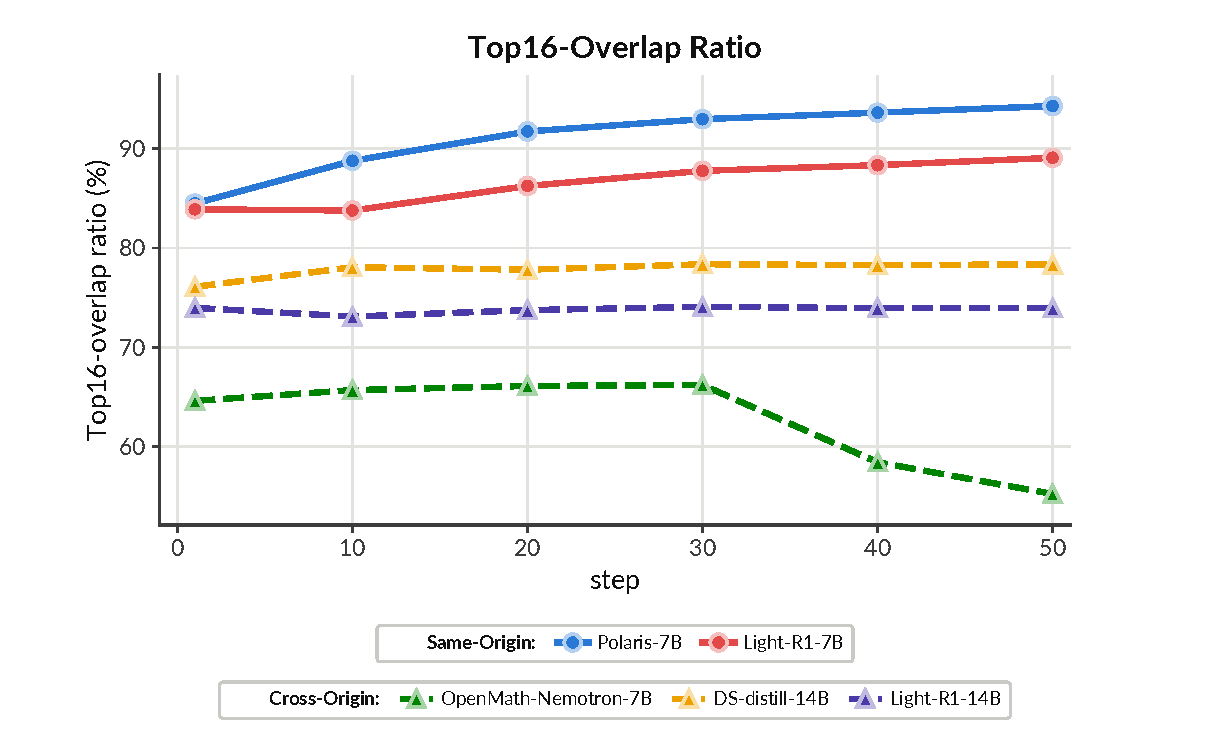
\includegraphics[width=\linewidth]{latex/figures/discussion/to_dpsk7b_top16_overlap.pdf}
        \caption{DS-distill-7B OPD 实验}
    \end{subfigure}

    \caption{不同OPD实验中教师模型与学生模型的Top-K（K=16）重叠比率。图(a)和图(b)中的学生模型分别为DS-distill-1.5B和DS-distill-7B。实线表示使用同原点教师模型的OPD实验；虚线表示使用不同原点教师模型的OPD实验。}
    \label{fig:top16_overlap_ratio}
\end{figure*}

\begin{figure}[htbp]
    \centering
    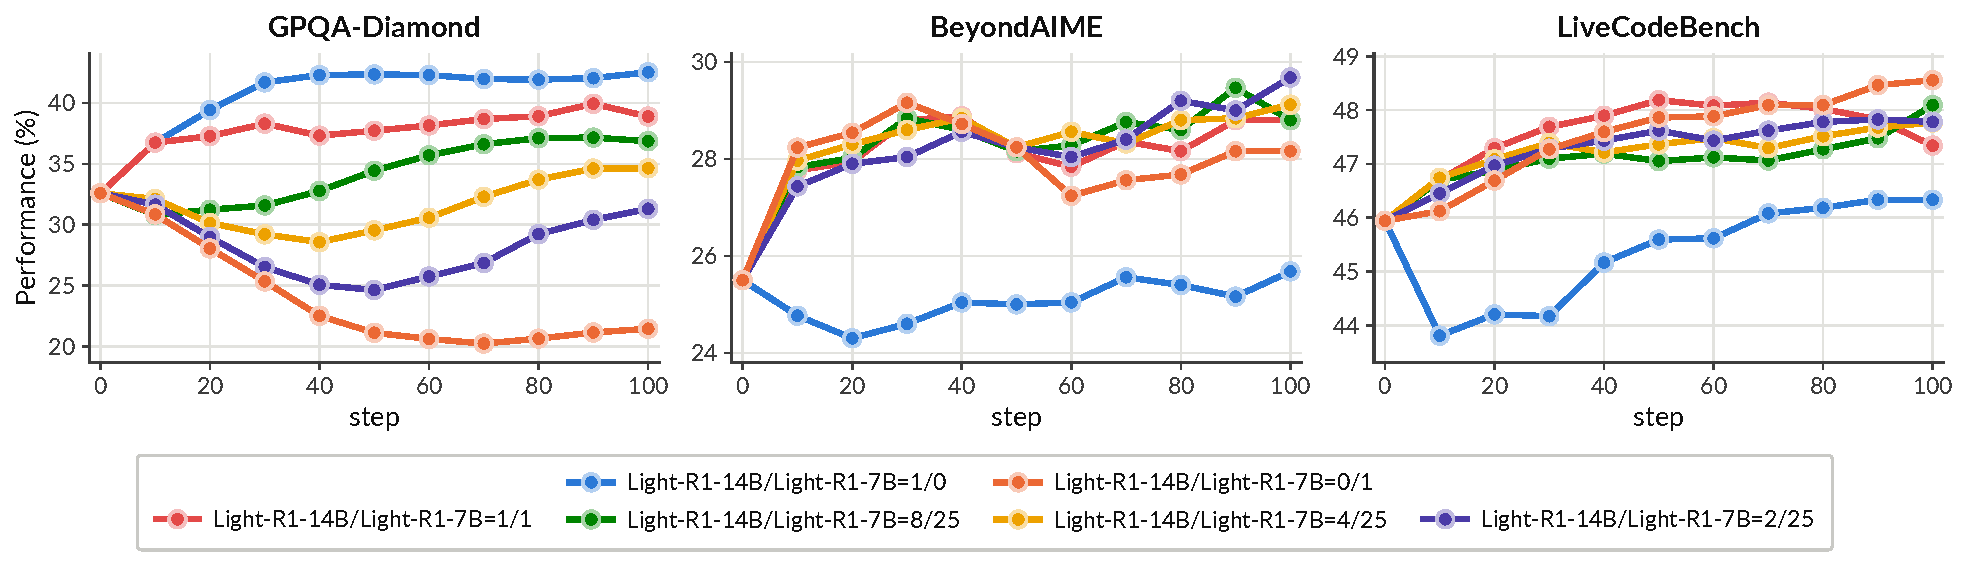
\includegraphics[width=0.99\linewidth]{latex/figures/discussion/mopd_light_14b_7b_panel.pdf}
    \caption{DS-distill-7B（学生）的MOPD实验结果，以及Light-R1-7B（数学教师）和Light-R1-14B（科学/推理教师）的实验结果。图例表示不同MOPD实验中专家数据混合比例（Light-R1-14B/Light-R1-7B $\in\{1/0, 1/1, 8/25, 4/25, 2/25, 0/1\}$ ）。}
    \label{fig:mopd_7b}
\end{figure}

在整篇论文中，模型原点始终是区分广泛泛化与狭窄拟合的最关键因子。我们最后通过两项分析更直接地探讨了原因：一是OPD如何在训练过程中重塑学生模型的策略，二是在MOPD中同源教师与异源教师竞争时，这种影响的具体表现。

\paragraph{同源OPD将学生的策略作为一个整体进行对齐。}
为了探究 OPD 如何在训练损失之外改变学生策略，我们测量了在训练过程中教师与学生下一个 token 分布之间的 top-$K$ ($K{=}16$ ) 重叠比率~\citep{li2026rethinking}（见图~\ref{fig:top16_overlap_ratio}）。
1.5B 和 7B 的学生均表现出两种一致的模式。
首先，相同原点的教师对应的重叠比率明显高于跨原点的情况，这证实了在任何 OPD 之前，共享原点已使学生策略更接近教师策略。
其次，更具启示性的是，相同原点的重叠比率在训练过程中显著上升，而跨原点的重叠比率则保持平稳甚至下降。
由于两种情景都最小化相同的教师-学生 KL 目标，这一对比表明：相同原点的 OPD 逐步实现学生对教师策略的全面对齐，而跨原点的 OPD 仅在训练分布上减少散度，却未能促使两策略达成更广泛的共识。
这为“相同原点可泛化，跨原点仅拟合”提供了机制解释：广泛迁移源于整体策略对齐，而这种对齐在教师与学生共享原点时更容易实现。

\paragraph{同源教师在MOPD中产生的引力更强。}
当将同源教师与跨源教师结合时，同样的不对称性再次显现。我们在 DS-distill-7B 上重复了 MOPD 实验，使用同源的 Light-R1-7B 作为数学教师，以及跨源的 Light-R1-14B 作为科学/IF 教师（图~\ref{fig:mopd_7b}）。在 GPQA-Diamond 上，即使在 $1{:}1$ 平衡混合比例下，科学教师获得相等份额，学生的科学准确率仍迅速向数学教师 Light-R1-7B 靠拢。结合上述对齐分析可知，在 MOPD 中，同源教师对学生的影响力强于跨源教师，因此教师之间的天平不仅受混合比例影响，还受到每个教师与学生原点接近程度的影响。

\begin{insightbox}
\textbf{要点：}
同源OPD在训练过程中提高了教师-学生模型的前$K$ 重叠度，而跨源OPD则没有，因此广泛泛化来自于整体对齐学生策略，而非仅仅降低在训练分布上的KL散度。因此，同源教师对学生的牵引力强于跨源教师，从而在起源和混合比例两个方面都倾斜了MOPD的天平。
\end{insightbox}